\documentclass[10pt,a4paper]{article}

% ===============================================================================
% PREAMBLE & PACKAGES
% ===============================================================================
\usepackage{fontspec}
\setmainfont{Latin Modern Roman}
\setmonofont{Latin Modern Mono}
\usepackage{unicode-math}
\setmathfont{Latin Modern Math}

\usepackage[margin=0.7in,top=0.9in,bottom=0.9in]{geometry}
\usepackage{xcolor}
\usepackage{tikz}
\usetikzlibrary{shapes.geometric, arrows.meta, positioning, calc, fit, decorations.pathreplacing}
\usepackage[most]{tcolorbox}
\usepackage{tabularx}
\usepackage{array}
\usepackage{enumitem}
\usepackage{amsmath}
\usepackage{fancyhdr}
\usepackage{microtype}
\usepackage[colorlinks=true,linkcolor=myteal,citecolor=mypurple,urlcolor=myblue]{hyperref}

\hyphenpenalty=10000
\exhyphenpenalty=10000
\sloppy

% ===============================================================================
% COLOR PALETTE (Strict adherence to spec)
% ===============================================================================
\definecolor{myred}{RGB}{196,30,58}       % section headings
\definecolor{mydark}{RGB}{30,30,50}       % body text
\definecolor{mygreen}{RGB}{14,120,80}     % definition boxes
\definecolor{myteal}{RGB}{0,130,140}      % formula boxes, diagrams, subsection headings
\definecolor{myamber}{RGB}{180,100,0}     % example boxes
\definecolor{mypurple}{RGB}{100,30,160}   % exam/viva boxes
\definecolor{myblue}{RGB}{25,90,170}      % hyperlinks/diagrams
\definecolor{mygray}{RGB}{246,247,249}    % tikzbox background
\definecolor{mgframe}{RGB}{180,185,200}   % tikzbox border
\definecolor{watermark}{RGB}{145,150,170} % footer watermark

\definecolor{hdrred}{RGB}{250,232,235}
\definecolor{hdrgreen}{RGB}{220,244,233}
\definecolor{hdrteal}{RGB}{220,242,244}
\definecolor{hdramber}{RGB}{253,242,215}
\definecolor{hdrpurple}{RGB}{238,228,255}
\definecolor{hdrblue}{RGB}{235,242,250}

% ===============================================================================
% TCOLORBOX STYLES
% ===============================================================================
\tcbset{
  tikzbox/.style={colback=mygray, colframe=mgframe, boxrule=0.6pt, arc=4pt,
    left=8pt, right=8pt, top=6pt, bottom=6pt,
    colbacktitle=mgframe, coltitle=mydark, fonttitle=\small\bfseries},
  defbox/.style={colback=hdrgreen, colframe=mygreen, boxrule=0.8pt, arc=4pt,
    left=9pt, right=9pt, top=6pt, bottom=6pt,
    colbacktitle=mygreen, coltitle=white, fonttitle=\small\bfseries},
  formulabox/.style={colback=hdrteal, colframe=myteal, boxrule=0.8pt, arc=4pt,
    left=9pt, right=9pt, top=7pt, bottom=7pt,
    colbacktitle=myteal, coltitle=white, fonttitle=\small\bfseries},
  examplebox/.style={colback=hdramber, colframe=myamber, boxrule=0.8pt, arc=4pt,
    left=9pt, right=9pt, top=6pt, bottom=6pt,
    colbacktitle=myamber, coltitle=white, fonttitle=\small\bfseries},
  masonbox/.style={colback=hdrpurple, colframe=mypurple, boxrule=0.8pt, arc=4pt,
    left=9pt, right=9pt, top=6pt, bottom=6pt,
    colbacktitle=mypurple, coltitle=white, fonttitle=\small\bfseries},
  exambox/.style={colback=hdrpurple, colframe=mypurple, boxrule=1pt, arc=5pt,
    left=10pt, right=10pt, top=8pt, bottom=8pt,
    colbacktitle=mypurple, coltitle=white, fonttitle=\bfseries,
    title after break={\textbf{Frequently Asked / Viva Questions (contd.)}}}
}
\tcbset{breakable}

% ===============================================================================
% TIKZ STYLES
% ===============================================================================
\tikzset{
  block/.style={rectangle, draw=myteal, fill=hdrteal, text width=2.4cm, align=center, minimum height=0.95cm, font=\small, rounded corners=3pt, line width=0.7pt},
  arrow/.style={-Stealth, thick, color=mydark},
  line/.style={thick, color=mydark}
}

% ===============================================================================
% MACROS & COMMANDS
% ===============================================================================
\newcommand{\Q}[1]{\textbf{#1}\par\vspace{2pt}}
\newcolumntype{Y}{>{\raggedright\arraybackslash}X}
\newcolumntype{C}{>{\centering\arraybackslash}X}

% Header & Footer
\pagestyle{fancy}
\fancyhf{}
\fancyhead[L]{\small\color{mydark}\textbf{OE-EC804B} --- Microwave Integrated Circuits}
\fancyhead[R]{\small\color{myteal}\textbf{Module 4 Notes}}
\fancyfoot[C]{\small\color{mydark}\thepage}
\fancyfoot[R]{\small\color{watermark}\copyright\ Biraj Sarkar}
\renewcommand{\headrulewidth}{0.6pt}

\hypersetup{pdftitle={OE-EC804B Module 4 Exam Notes}}

\begin{document}

% ===============================================================================
% TITLE BLOCK
% ===============================================================================
\begin{center}
  {\LARGE\bfseries\color{myred} OE-EC804B --- Microwave Integrated Circuits}\\[5pt]
  {\normalsize\color{mydark} Semester VIII \quad$\bullet$\quad 3L:0T:0P \quad$\bullet$\quad 3 Credits}\\[3pt]
  {\normalsize\color{myteal}\textbf{Module 4 Exam Notes: Parallel-Coupled Lines \& Power Dividers}}\\[3pt]
  {\small\color{mydark} CGEC \;$|$\; B.Tech ECE (2023--27) \;$|$\; \textit{Biraj Sarkar}}
\end{center}
\vspace{2pt}
\noindent{\color{myred}\rule{\linewidth}{1.5pt}}
\vspace{2pt}

\hypersetup{linkcolor=mydark}
\tableofcontents
\hypersetup{linkcolor=myteal}
\newpage

% ===============================================================================
% 1. PARALLEL-COUPLED MICROSTRIP LINES
% ===============================================================================
\section{Parallel-Coupled Microstrip Lines}

Coupled microstrip lines consist of two unshielded, parallel microstrip conductors of width $W$ separated by a gap distance $S$ on a dielectric substrate of thickness $h$. When electromagnetic signals travel on one line, energy is coupled to the adjacent line via fringing electric and magnetic fields.

\subsection{Even-Mode and Odd-Mode Analysis}
Any arbitrary voltage and current excitation on two symmetrical coupled lines can be decomposed into two fundamental orthogonal modes:

\begin{enumerate}[leftmargin=*, itemsep=5pt]
  \item \textbf{Even Mode ($+ +$):} Both conductors are excited with equal amplitude and equal phase ($V_1 = V_2 = V_e, I_1 = I_2 = I_e$). No net current flows across the central plane of symmetry. The symmetry plane acts as an \textbf{ideal magnetic wall ($\partial E/\partial n = 0, H_{tan} = 0$)}.
  \item \textbf{Odd Mode ($+ -$):} Conductors are excited with equal amplitude but opposite phase ($V_1 = -V_2 = V_o, I_1 = -I_2 = I_o$). The zero-voltage plane of symmetry acts as an \textbf{ideal electric wall ($E_{tan} = 0$)}.
\end{enumerate}

\subsection{Characteristic Impedances (\texorpdfstring{$Z_{0e}, Z_{0o}$}{Z0e, Z0o}) \& Coupling Equations}

\begin{tcolorbox}[formulabox, title={Coupled Line Impedance \& Coupling Formulas}]
  The system characteristic impedance $Z_0$ and voltage coupling coefficient $C$ are uniquely determined by even-mode impedance $Z_{0e}$ and odd-mode impedance $Z_{0o}$:
  \begin{equation}
    Z_0 = \sqrt{Z_{0e} \cdot Z_{0o}} \quad ; \quad C = \frac{Z_{0e} - Z_{0o}}{Z_{0e} + Z_{0o}}
  \end{equation}
  Inverting these relations yields design formulas for $Z_{0e}$ and $Z_{0o}$ given $Z_0$ and coupling factor $C$:
  \begin{equation}
    Z_{0e} = Z_0 \sqrt{\frac{1+C}{1-C}} \quad ; \quad Z_{0o} = Z_0 \sqrt{\frac{1-C}{1+C}}
  \end{equation}
\end{tcolorbox}

\subsection{Quarter-Wave Coupling Region Length}
For a single-section coupled line directional coupler, maximum power coupling occurs when the physical length $L$ of the coupled region is a quarter guided wavelength ($\lambda_g/4$):
\begin{equation}
  L = \frac{\lambda_g}{4} = \frac{c}{4 f \sqrt{\varepsilon_{eff,avg}}} \quad \text{where } \varepsilon_{eff,avg} \approx \frac{\varepsilon_{eff,e} + \varepsilon_{eff,o}}{2}
\end{equation}

\begin{tcolorbox}[examplebox, title={Worked Numerical: $10\text{ dB}$ Coupled Line Design}]
  \textbf{Problem:} Design a $10\text{ dB}$ microstrip directional coupler in a $50\text{ }\Omega$ system. Calculate the required even-mode ($Z_{0e}$) and odd-mode ($Z_{0o}$) characteristic impedances.
  \tcblower
  \textbf{Solution:}
  \begin{enumerate}[label=Step \arabic*:, itemsep=4pt]
    \item Convert coupling factor $C_{\text{dB}} = 10\text{ dB}$ to voltage coupling ratio $C$:
      \begin{equation}
        \begin{aligned}
          C_{\text{dB}} &= 20 \log_{10}\left(\frac{1}{C}\right) = 10 \implies \log_{10}(C) = -0.5 \\
          &\implies C = 10^{-0.5} = 0.3162
        \end{aligned}
      \end{equation}
    \item Calculate $Z_{0e}$ and $Z_{0o}$ for $Z_0 = 50\text{ }\Omega$:
      \begin{equation}
        \begin{aligned}
          Z_{0e} &= 50 \sqrt{\frac{1 + 0.3162}{1 - 0.3162}} = 50 \sqrt{\frac{1.3162}{0.6838}} \\
          &= 50 \sqrt{1.9248} = 50 \times 1.3874 = 69.37\text{ }\Omega
        \end{aligned}
      \end{equation}
      \begin{equation}
        Z_{0o} = 50 \sqrt{\frac{1 - 0.3162}{1 + 0.3162}} = 50 \sqrt{0.5195} = 50 \times 0.7208 = 36.04\text{ }\Omega
      \end{equation}
    \item Check consistency: $Z_0 = \sqrt{Z_{0e} Z_{0o}} = \sqrt{69.37 \times 36.04} = \sqrt{2500} = 50.0\text{ }\Omega$ (Correct!).
  \end{enumerate}
\end{tcolorbox}

% ===============================================================================
% 2. BRANCH-LINE COUPLER AND RAT-RACE HYBRID RING
% ===============================================================================
\section{Branch-Line Coupler and Rat-Race Hybrid Ring}

\subsection{Branch-Line Power Divider ($3\text{ dB}$, $90^\circ$ Quadrature Hybrid)}
A \textbf{Branch-Line Coupler} is a 4-port symmetrical directional coupler consisting of four $\lambda_g/4$ microstrip arms forming a rectangular ring.

\begin{tcolorbox}[masonbox, title={Branch-Line Coupler Design Parameters}]
  For a $3\text{ dB}$ equal power split in a $50\text{ }\Omega$ system ($Z_0 = 50\text{ }\Omega$):
  \begin{itemize}[leftmargin=*, noitemsep]
    \item Horizontal main series arms impedance: $Z_A = \frac{Z_0}{\sqrt{2}} = \frac{50}{\sqrt{2}} \approx 35.35\text{ }\Omega$.
    \item Vertical shunt branch arms impedance: $Z_B = Z_0 = 50\text{ }\Omega$.
    \item All 4 branch lengths are exactly $L = \lambda_g/4$.
  \end{itemize}
\end{tcolorbox}

\subsubsection{Scattering Matrix ($[S]$) of Branch-Line Coupler}
When signal is fed at Port 1, power splits equally between Port 2 ($0^\circ$) and Port 3 ($-90^\circ$), while Port 4 is fully isolated ($S_{41} = 0$):
\begin{equation}
  [S]_{\text{Branch-Line}} = -\frac{1}{\sqrt{2}} \begin{bmatrix} 0 & j & 1 & 0 \\ j & 0 & 0 & 1 \\ 1 & 0 & 0 & j \\ 0 & 1 & j & 0 \end{bmatrix}
\end{equation}

\subsection{Rat-Race Hybrid Ring ($180^\circ$ Hybrid)}
A \textbf{Rat-Race Coupler} consists of a circular microstrip ring of total perimeter $1.5\lambda_g$ ($6\theta = 540^\circ$) with 4 ports. Ports 1, 2, 3, and 4 are separated by $\lambda_g/4$ gaps, except between Port 3 and Port 4 which are separated by a $3\lambda_g/4$ gap.

\begin{tcolorbox}[formulabox, title={Rat-Race Impedance \& Scattering Matrix}]
  Ring characteristic impedance: $Z_{\text{ring}} = \sqrt{2} Z_0 \approx 70.7\text{ }\Omega$ (for $Z_0 = 50\text{ }\Omega$).
  \begin{equation}
    [S]_{\text{Rat-Race}} = -\frac{j}{\sqrt{2}} \begin{bmatrix} 0 & 1 & 0 & -1 \\ 1 & 0 & 1 & 0 \\ 0 & 1 & 0 & 1 \\ -1 & 0 & 1 & 0 \end{bmatrix}
  \end{equation}
  \begin{itemize}[leftmargin=*, noitemsep]
    \item \textbf{Sum Port ($\Sigma$ / Port 1):} Input at Port 1 splits equally in-phase ($0^\circ$) between Ports 2 and 4. Port 3 is isolated due to destructive interference ($180^\circ$ path difference).
    \item \textbf{Difference Port ($\Delta$ / Port 3):} Input at Port 3 splits equally out-of-phase ($180^\circ$) between Ports 2 and 4. Port 1 is isolated.
  \end{itemize}
\end{tcolorbox}

\begin{tcolorbox}[tikzbox, title={Topologies of Branch-Line Coupler ($90^\circ$) and Rat-Race Hybrid Ring ($180^\circ$)}]
\centering
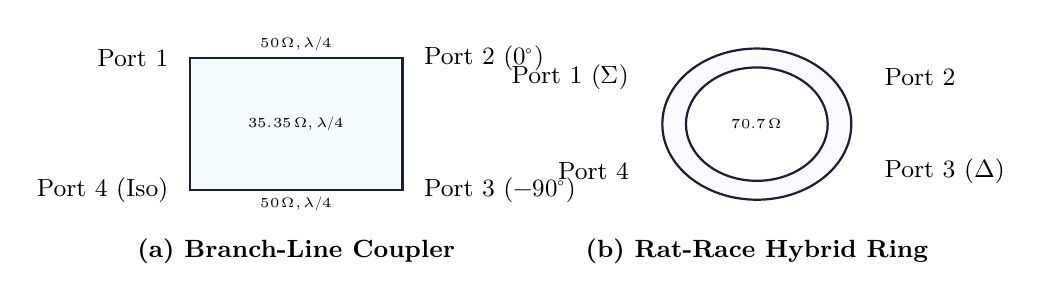
\begin{tikzpicture}[x=1.5cm, y=1.2cm]
  % Branch Line Coupler
  \draw[line, fill=hdrteal!30] (0,0) rectangle (1.8,1.4);
  \node at (0.9,0.7) {\tiny\textbf{$35.35\,\Omega, \lambda/4$}};
  \node at (0.9,1.55) {\tiny\textbf{$50\,\Omega, \lambda/4$}};
  \node at (0.9,-0.15) {\tiny\textbf{$50\,\Omega, \lambda/4$}};
  \node[anchor=east] at (-0.1,1.4) {\small Port 1};
  \node[anchor=west] at (1.9,1.4) {\small Port 2 ($0^\circ$)};
  \node[anchor=east] at (-0.1,0) {\small Port 4 (Iso)};
  \node[anchor=west] at (1.9,0) {\small Port 3 ($-90^\circ$)};
  \node[align=center] at (0.9,-0.65) {\small\textbf{(a) Branch-Line Coupler}};

  % Rat Race Hybrid Ring
  \draw[line, fill=hdrpurple!20] (4.8,0.7) circle (0.8);
  \draw[line, fill=white] (4.8,0.7) circle (0.6);
  \node at (4.8,0.7) {\tiny\textbf{$70.7\,\Omega$}};
  \node[anchor=east] at (3.8,1.2) {\small Port 1 ($\Sigma$)};
  \node[anchor=west] at (5.8,1.2) {\small Port 2};
  \node[anchor=west] at (5.8,0.2) {\small Port 3 ($\Delta$)};
  \node[anchor=east] at (3.8,0.2) {\small Port 4};
  \node[align=center] at (4.8,-0.65) {\small\textbf{(b) Rat-Race Hybrid Ring}};
\end{tikzpicture}
\end{tcolorbox}

% ===============================================================================
% QUICK REVISION PAGE
% ===============================================================================
\newpage
\begin{center}
  {\large\bfseries\color{myred} Quick Revision --- Module 4}\\[3pt]
  {\small\color{mydark} Parallel-Coupled Microstrip Lines \& Power Dividers $|$ OE-EC804B}
\end{center}
\noindent{\color{myred}\rule{\linewidth}{1.2pt}}
\vspace{4pt}

\begin{tcolorbox}[formulabox, title={\textbf{Key Concepts and Metrics at a Glance}}]
\renewcommand{\arraystretch}{1.35}
\begin{tabularx}{\linewidth}{>{\raggedright\arraybackslash\bfseries}p{4.5cm} X}
System Impedance $Z_0$ & $Z_0 = \sqrt{Z_{0e} \cdot Z_{0o}}$ \quad (Geometric mean of even and odd mode impedances) \\[4pt]
Voltage Coupling Factor $C$ & $C = \frac{Z_{0e} - Z_{0o}}{Z_{0e} + Z_{0o}} \implies Z_{0e} = Z_0 \sqrt{\frac{1+C}{1-C}}, Z_{0o} = Z_0 \sqrt{\frac{1-C}{1+C}}$. \\[4pt]
Branch-Line Arm Impedances & Main series arms $Z_A = Z_0 / \sqrt{2} = 35.35\text{ }\Omega$; Branch arms $Z_B = Z_0 = 50\text{ }\Omega$. \\[4pt]
Rat-Race Ring Impedance & Ring characteristic impedance $Z_{\text{ring}} = \sqrt{2} Z_0 = 70.7\text{ }\Omega$. \\[4pt]
Rat-Race Arm Spacings & 3 sections of $\lambda_g/4$ and 1 section of $3\lambda_g/4$ (Total perimeter $1.5\lambda_g$). \\
\end{tabularx}
\end{tcolorbox}

\begin{tcolorbox}[defbox, title={\textbf{One-Line Definitions}}]
  \begin{itemize}[leftmargin=*, noitemsep]
    \item \textbf{Even Mode ($Z_{0e}$):} Symmetrical mode where coupled line currents flow in identical directions with magnetic wall symmetry.
    \item \textbf{Odd Mode ($Z_{0o}$):} Anti-symmetrical mode where coupled line currents flow in opposite directions with electric wall symmetry.
    \item \textbf{Quadrature Hybrid ($90^\circ$):} Directional coupler providing equal power division with $90^\circ$ phase shift between output ports.
    \item \textbf{Rat-Race Ring ($180^\circ$):} 4-port hybrid ring providing equal in-phase ($0^\circ$) or anti-phase ($180^\circ$) power division.
  \end{itemize}
\end{tcolorbox}

\begin{tcolorbox}[exambox, title={\textbf{Frequently Asked / Viva Questions}}]
  \begin{enumerate}[topsep=0pt, label=\textbf{Q\arabic*.}, itemsep=5pt]
    \item \Q{Define even-mode and odd-mode impedances ($Z_{0e}, Z_{0o}$) of coupled microstrip lines.}
    $Z_{0e}$ is the characteristic impedance when lines are driven in-phase with equal currents. $Z_{0o}$ is the impedance when lines are driven out-of-phase with opposite currents.

    \item \Q{How is characteristic impedance $Z_0$ related to $Z_{0e}$ and $Z_{0o}$?}
    $Z_0 = \sqrt{Z_{0e} \cdot Z_{0o}}$.

    \item \Q{What is the physical length of a parallel-coupled microstrip directional coupler?}
    The coupled region length $L = \lambda_g/4$ at the center frequency.

    \item \Q{Explain the operation of a $3\text{ dB}$ Branch-Line Coupler.}
    A 4-port quadrature hybrid consisting of four $\lambda_g/4$ branches. Input at Port 1 splits equally between Port 2 ($0^\circ$) and Port 3 ($-90^\circ$), with Port 4 isolated.

    \item \Q{What are the arm impedances of a $50\text{ }\Omega$ Branch-Line Coupler?}
    The horizontal series arms have impedance $Z_0/\sqrt{2} = 35.35\text{ }\Omega$, and vertical shunt branch arms have impedance $Z_0 = 50\text{ }\Omega$.

    \item \Q{Describe the structure and port spacing of a Rat-Race Hybrid Ring.}
    A circular ring of characteristic impedance $\sqrt{2}Z_0 = 70.7\text{ }\Omega$ with 4 ports. Three port gaps are $\lambda_g/4$ and one gap is $3\lambda_g/4$ (total perimeter $1.5\lambda_g$).

    \item \Q{How does the Rat-Race coupler operate as a sum ($\Sigma$) and difference ($\Delta$) network?}
    Input at Port 1 splits in-phase ($0^\circ$) at Ports 2 and 4 ($\Sigma$ mode). Input at Port 3 splits out-of-phase ($180^\circ$) at Ports 2 and 4 ($\Delta$ mode).

    \item \Q{What causes directivity degradation in microstrip coupled lines?}
    Phase velocity mismatch between even mode ($\beta_e$) and odd mode ($\beta_o$), caused by non-homogeneous substrate/air dielectric boundary.

    \item \Q{How is crosstalk defined in parallel-coupled lines?}
    Crosstalk is unwanted electromagnetic power coupling from a driven primary line to an adjacent secondary signal line.

    \item \Q{What is the bandwidth restriction of branch-line and rat-race couplers?}
    They are narrowband components ($\approx 10\% - 20\%$ bandwidth) because their operation relies on exact $\lambda_g/4$ line lengths.
  \end{enumerate}
\end{tcolorbox}

\end{document}
